\chapter{数据和方法}

本研究尝试利用PcP-PKiKP震相组合来探测核幔边界的小尺度结构,包括界面起伏变化和其上方的速度异常,因此需要同时用到这两个震相的振幅和走时信息. CMB的起伏主要通过与标准模型的走时残差来约束,而其物性变化主要依靠PKiKP/PcP的振幅比来推断. 获得这两种信息都需要观测记录上出现可识别的震相,然而在一道地震记录上同时观测到PcP和PKiKP信号是比较困难的. 首先,对于PKiKP,由于较小的反射系数(图\ref{fig:rtf}b)加之噪声的干扰,其观测难度要远大于常规的核震相;其次,能观测到清晰PcP震相的震中距常常比较有限,在小震中距情况下,PcP的反射系数较小(图\ref{fig:rtf}a),而且容易受到S波及其尾波的干扰,因此比较合适的观测区间大致位于30{\textdegree}--40{\textdegree}. 因此,采用台阵叠加方法寻找和识别弱信号则非常有必要. 本章主要介绍研究所用到的数据来源、全球的PKiKP和PcP观测情况,以及包括PWS在内的数据处理方法和振幅比、走时残差测量和可靠性评价方法. 


\begin{figure}[!ht]
		\centering
%		\subfloat[][]{\label{fig:cmb}%
%		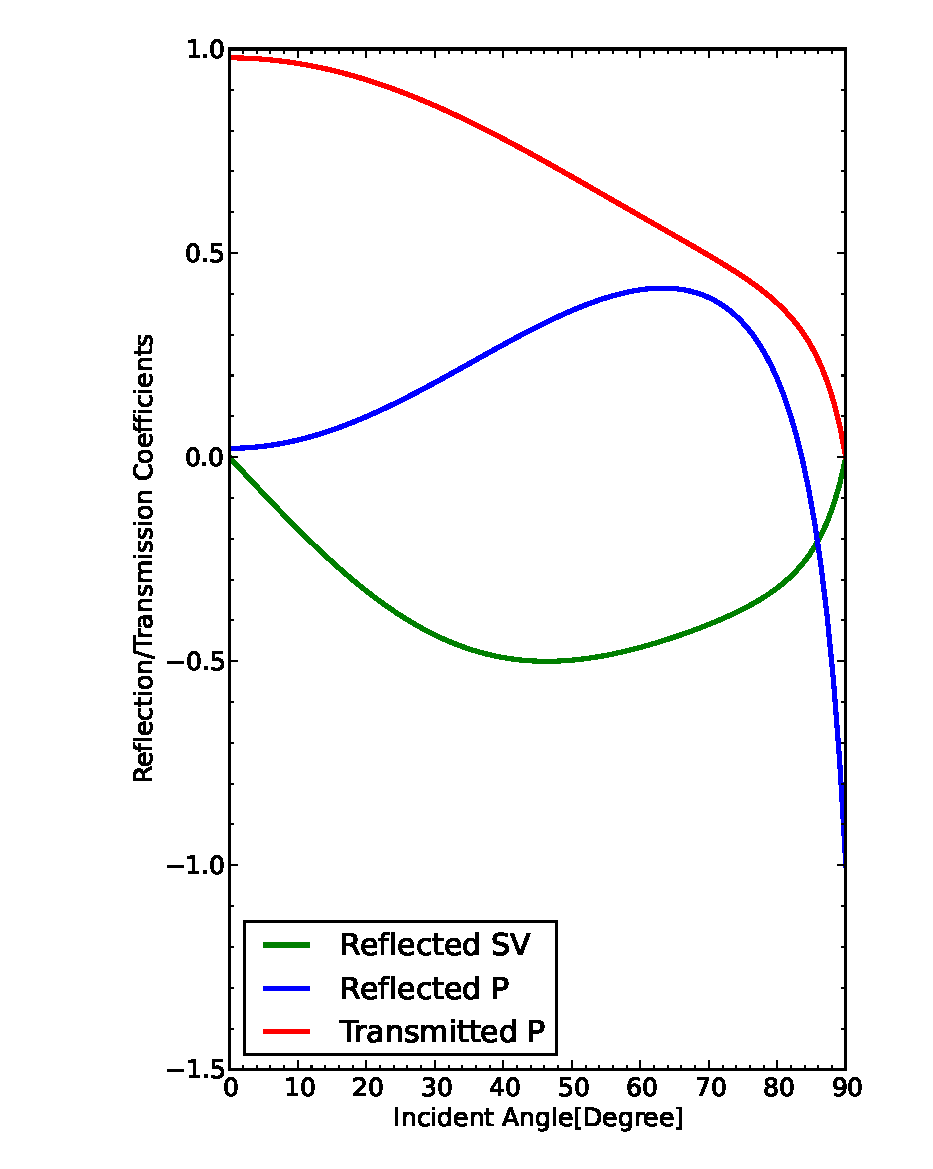
\includegraphics[width=0.45\linewidth]{fig/chap2/cmb.eps}
%}			
%		%\hspace{2em}
%		\subfloat[][]{\label{fig:icb}%
%		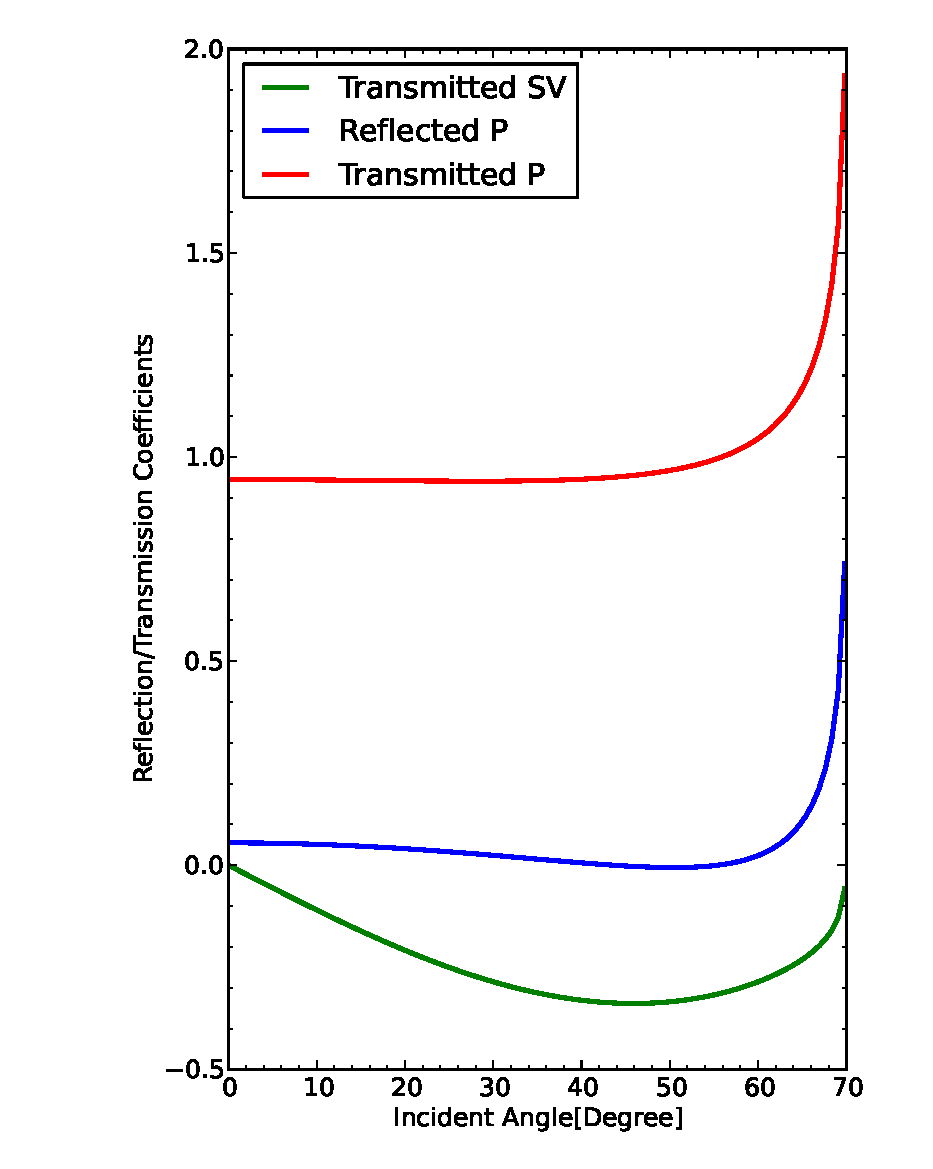
\includegraphics[width=0.45\linewidth]{fig/chap2/icb.eps}
%}		
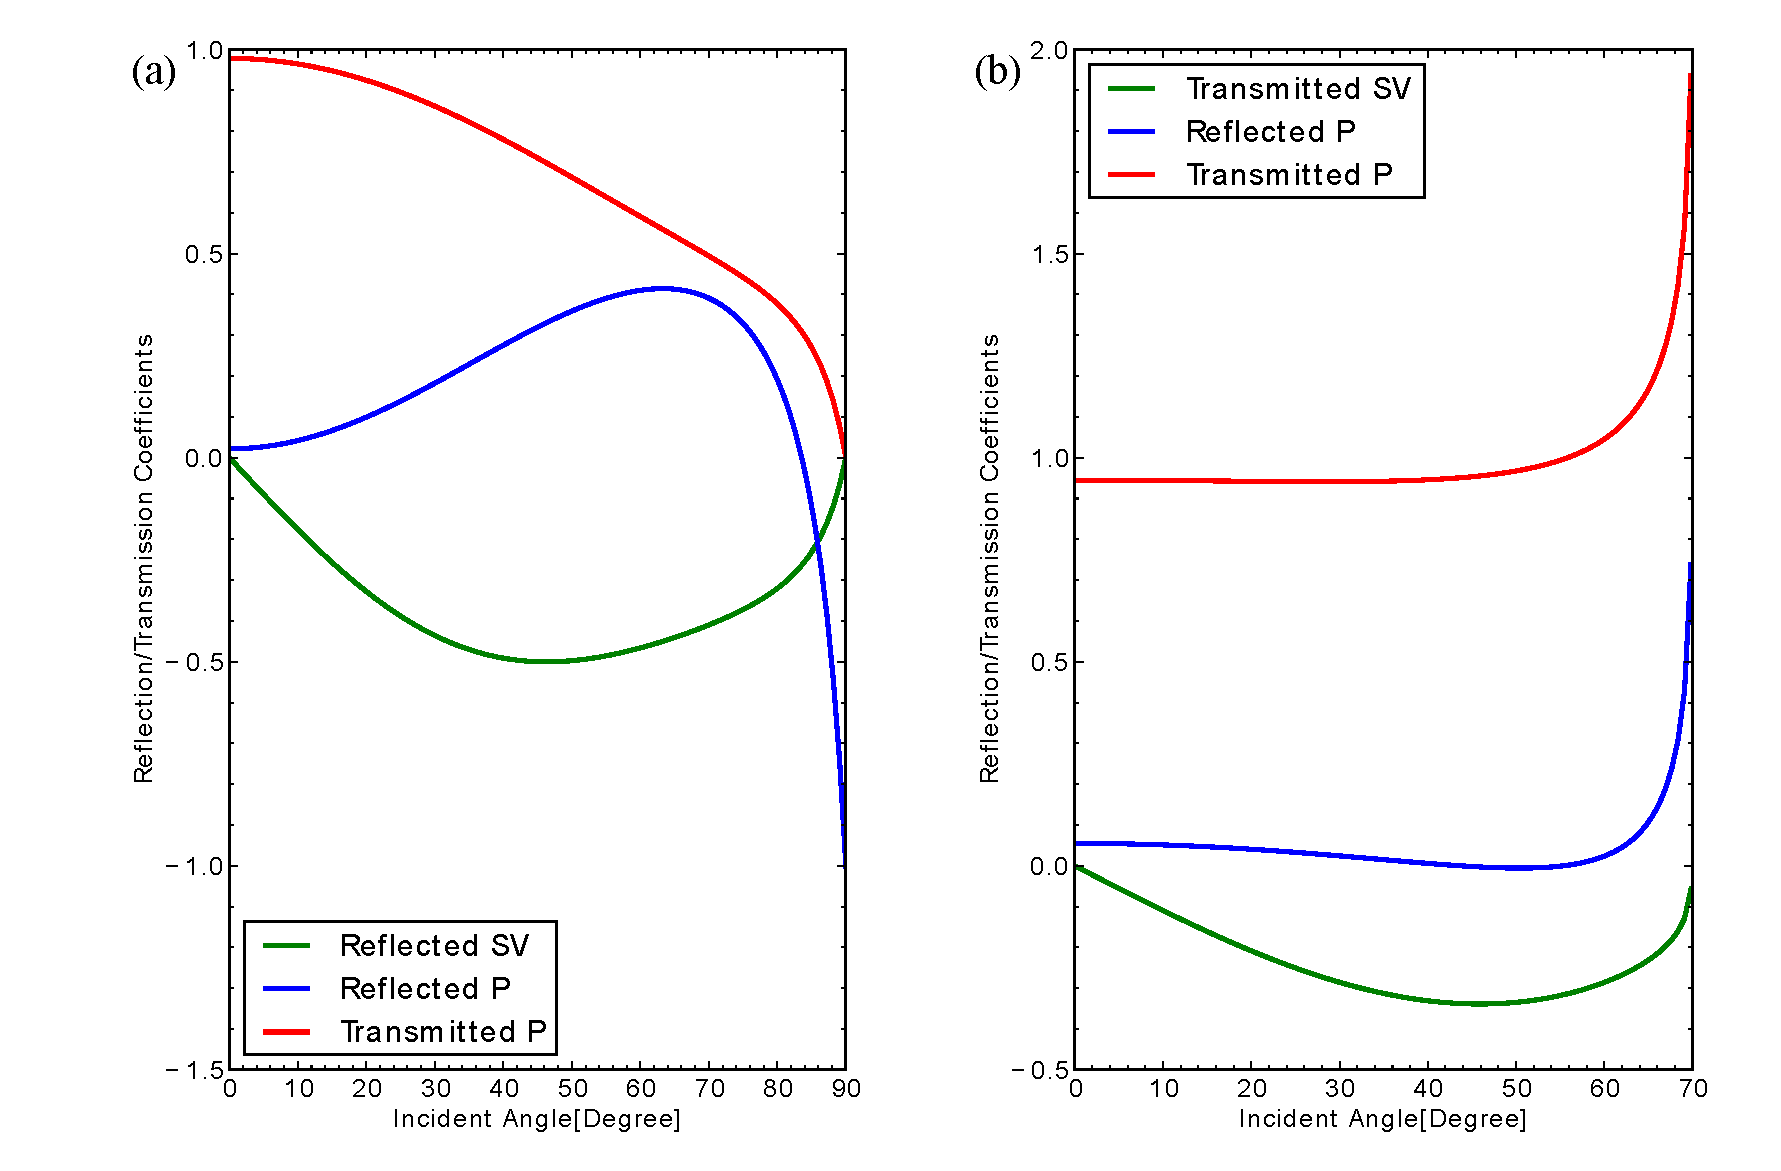
\includegraphics[width=0.9\linewidth]{fig/chap2/cmb_icb.eps}
		\caption{根据PREM计算的(a)~CMB和(b)~ICB 的P波反射、透射系数. 与透射和转换P波系数相比,PKiKP的反射系数非常小;而PcP反射系数大约在入射角为60{\textdegree}左右时取得最大. }
		\label{fig:rtf}
\end{figure}


\section{数据来源}

本硕士论文的前期工作主要是在全球范围内寻找PKiKP震相,然后从观测到PKiKP信号的地震记录中挑选出含有可识别PcP信号的记录. 数据的来源有(1)在IRIS上可下载的全球IMS小口径台阵数据;(2)日本Hi-net台网;(3)
国家测震台网,数据从国家测震台网数据备份中心(State Earthquake Information Service-Data Management Center)得到;(4)美国USArray. 数据来源的具体分布见图\ref{fig:data_source},可以看出由于台站分布的南北不均匀性,南半球的CMB和ICB的采样较少,只有澳大利用几个小口径台阵的数据. 

\begin{figure}
\centering
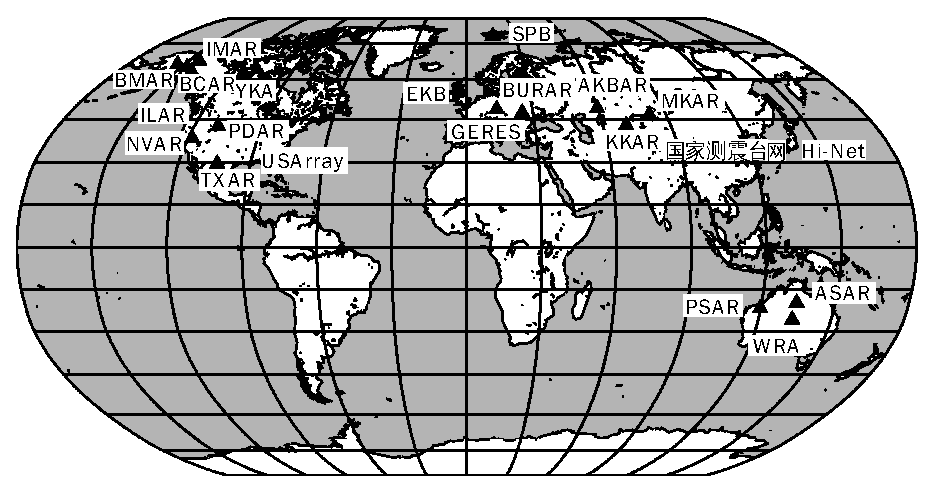
\includegraphics[width=0.8\linewidth]{fig/chap2/data_source}
\caption{本研究所收集PKiKP和PcP观测记录的数据来源分布. 包括全球范围分布的IMS小口径台阵,还有国家测震台网等大型密集台网. }
\label{fig:data_source}
\end{figure}

\subsection{IMS小口径台阵}

对于IMS小口径台阵,IRIS上大部分可下载数据的时间范围从2000至2015年,因此搜索的地震事件也基本在这个
时间范围,数据并不与之前的研究重合~\citep{Koper2004a}. 筛选的地震事件震级均大于Mw5.0,以保
证能产生可观测的PKiKP信号;地震的深度不加限制,因为IMS均为用于核爆监测目的的短周期台站,PKiKP
记录并不会受到浅源地震产生的面波的显著干扰;震中距范围从10{\textdegree}--50{\textdegree}. 利用IMS台阵数据做对比分析是本研究的主要内容,但从全球范围来看适合的台阵对并不多. 首先,台阵的分布很
不均匀,目前半数都位于北美,包括阿拉斯加的BCAR,BMAR,IMAR和ILAR;加拿大的Yellow Knife(YKA);
美国的NVAR,PDAR和TXAR. 而要满足相近震中距条件,再加上地震位置的限制,使得能够用来进行对照分析的台
阵组合仅有阿拉斯加的四个小口径台阵,美国的PDAR-NVAR和澳大利亚的WRA-ASAR. 位于中亚和欧洲的台阵有的没有
与之成对的台阵;有些由于震中距比较大(>50{\textdegree})和较低的信噪比,不能同时记录到同一地震事件
产生的PKiKP和PcP信号. 因此,本文集中讨论北美和澳大利亚IMS台阵的观测. 

\begin{table}[ht]
	\centering
	\caption{本文搜集PcP和PKiKP所用到的IMS小口径台阵}
	\begin{tabular}{*{5}{c}}
\hline
台阵 & 台站数 & 纬度\textsuperscript{*}(\textdegree) & 经度\textsuperscript{*}(\textdegree) & 数据起止日期\\
\hline
AKBAR & 9 & 49.2 & 59.9 & 2003.12--2015.09\\
MKAR & 10 & 46.7 & 82.3 & 2000.09--2015.09\\
KKAR & 9 & 43.1 & 70.5 & 2001.12--2015.09\\
BCAR & 5 & 63.0 & -141.8 & 2013.11--\\
BMAR & 5 & 67.4 & -144.5 & 2013.11--\\
IMAR & 5 & 66.0 & -153.7 & 2013.11--\\
ILAR & 19 & 64.7 & -146.9 & 1998.03--\\
YKA & 18 & 62.5 & -114.6 & 2005.09--\\
NVAR & 11 & 38.4 & -118.3 & 2003.07--\\
PDAR & 14 & 42.7 & -109.5 & 1998.03--\\
TXAR & 10 & 23.3 & -103.6 & 2000.04--\\
GERES & 24 & 48.8 & 13.7 & 2001.08--2002.03\\
BURAR & 9 & 47.6 & 25.2 & 2007.09--\\
EKB & 21 & -3.1 & 55.3 & 2014.03--\\
WRA & 26 & -19.9 & 134.4 & 2005.01--\\
ASAR & 19 & -23.6 & 133.9 & 2003.08--\\
PSAR & 13 & -21.5 & 119.8 & 2011.01--\\
SPB & 5 & 78.1 & 16.3 & 2009.03--\\
\hline
\multicolumn{5}{l}{\textsuperscript{*}\footnotesize{台阵的经纬度仅保留至一位小数}}
	\end{tabular}
\label{array}
\end{table}

每个IMS台阵基本由10到25个短周期台站组成(表\ref{array}),但有几个台阵例外,例如BCAR,BMAR和IMAR,它们在IRIS上的可用数据只从2013年才开始,尽管如此,它们也能为本研究补充一定的PcP和PKiKP观测. 
从所有可用数据中一共找到300个观测到PKiKP信号的台阵-事件对,从数据的分布来看,PKiKP观测集中在北美和澳大利亚区域,中亚和欧洲台阵的观测比较稀疏,这也和这些区域地震活动性不强有关(图\ref{fig:gl_pkikp}),从这些数据中再进行挑选得到同时观测到PcP和PKiKP的仅127对. 即使搜索了超过一万个地震的的数据,所找到的有效PKiKP数量仍然不多,这也表现出PKiKP弱振幅的本质并且其可观测性强烈依赖于环境噪声和台站状态. 尽管如此,利用这些小口径台阵还是能得到很多高质量的PcP和PKiKP观测,即不用做任何额外处理即可在全部台站的记录上看到这两个信号.

\begin{figure}
\centering
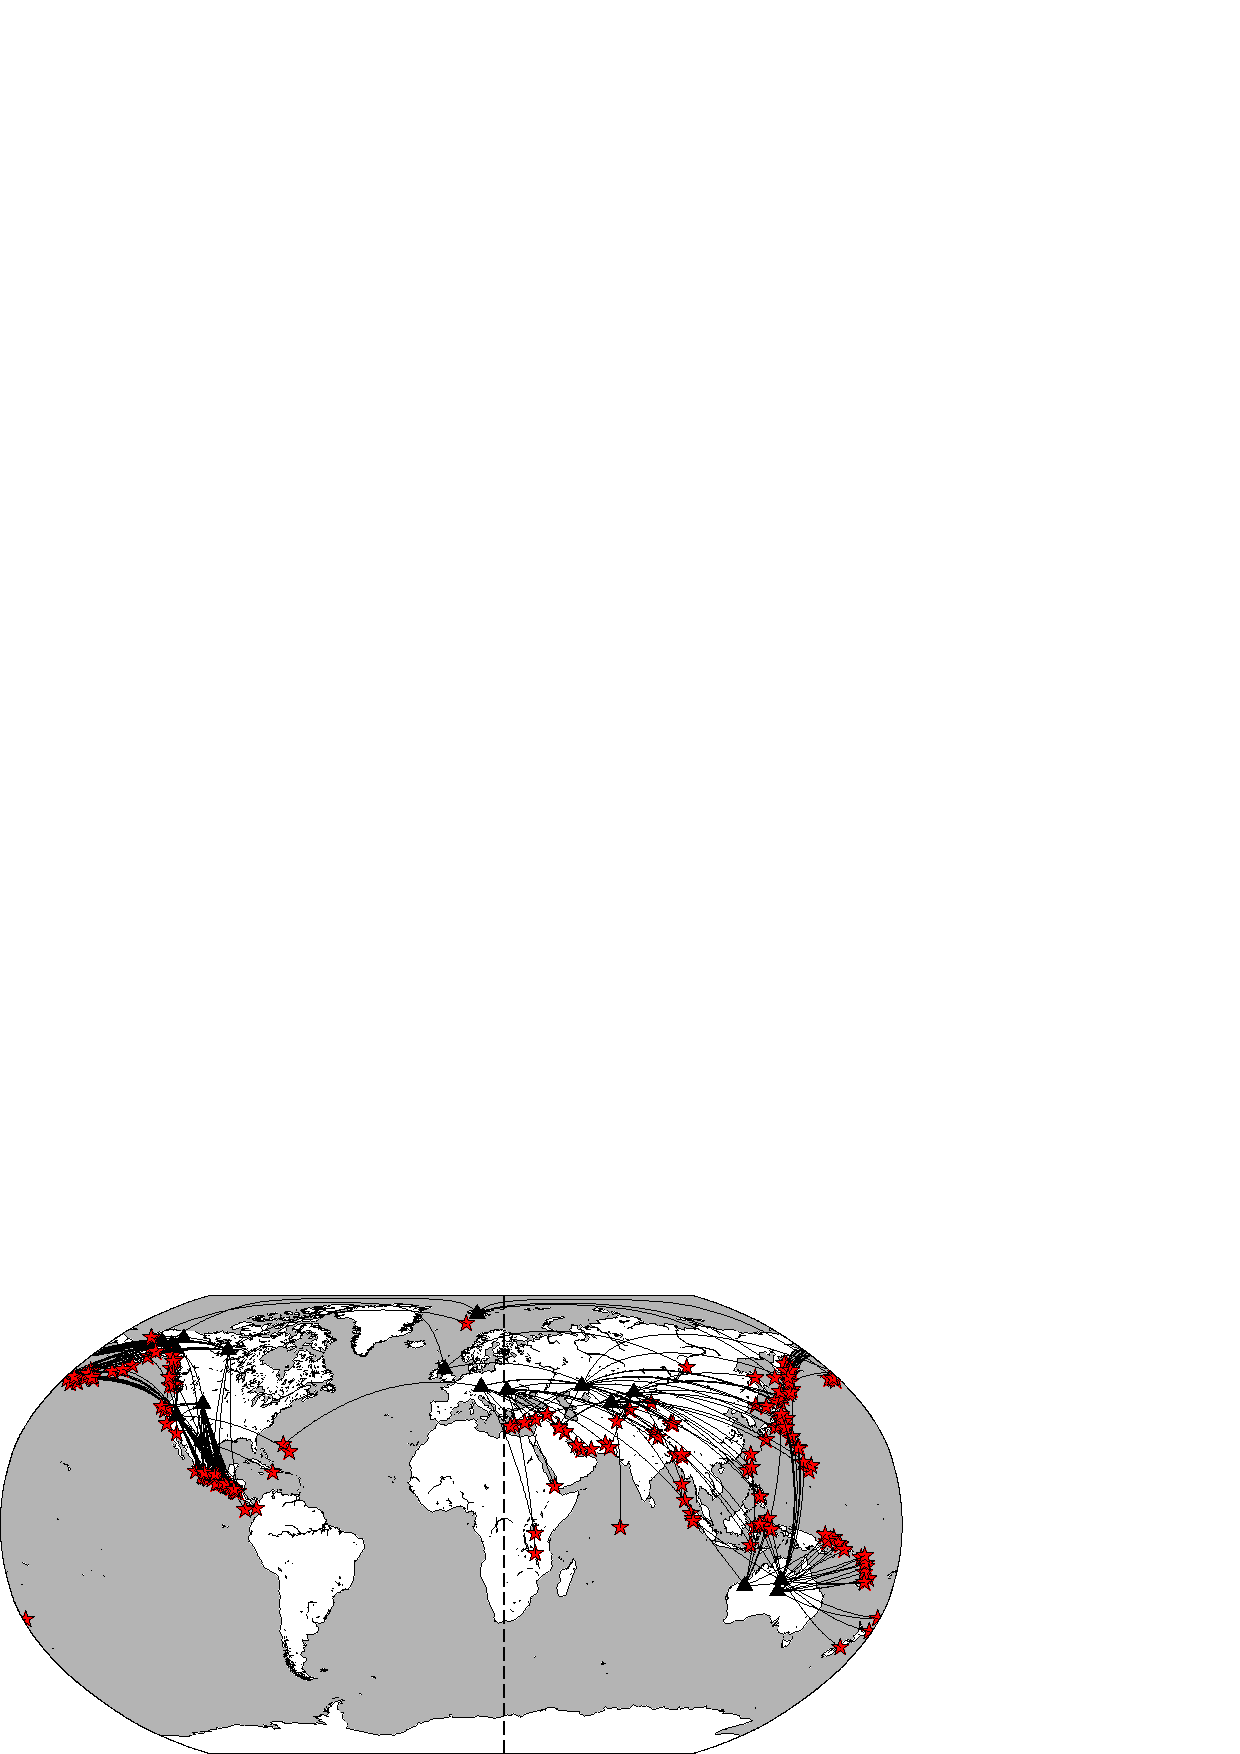
\includegraphics[width=0.8\linewidth]{fig/chap2/gl_pkikp}
\caption{利用全球IMS小口径台阵获得了300对可观测到PKiKP信号的事件-台阵对. 虚线为~\citet{Tanaka1997}定义的准东西半球分界线. 红色五角星为地震,黑色三角形表示IMS台阵. }
\label{fig:gl_pkikp}
\end{figure}

\begin{figure}
\centering
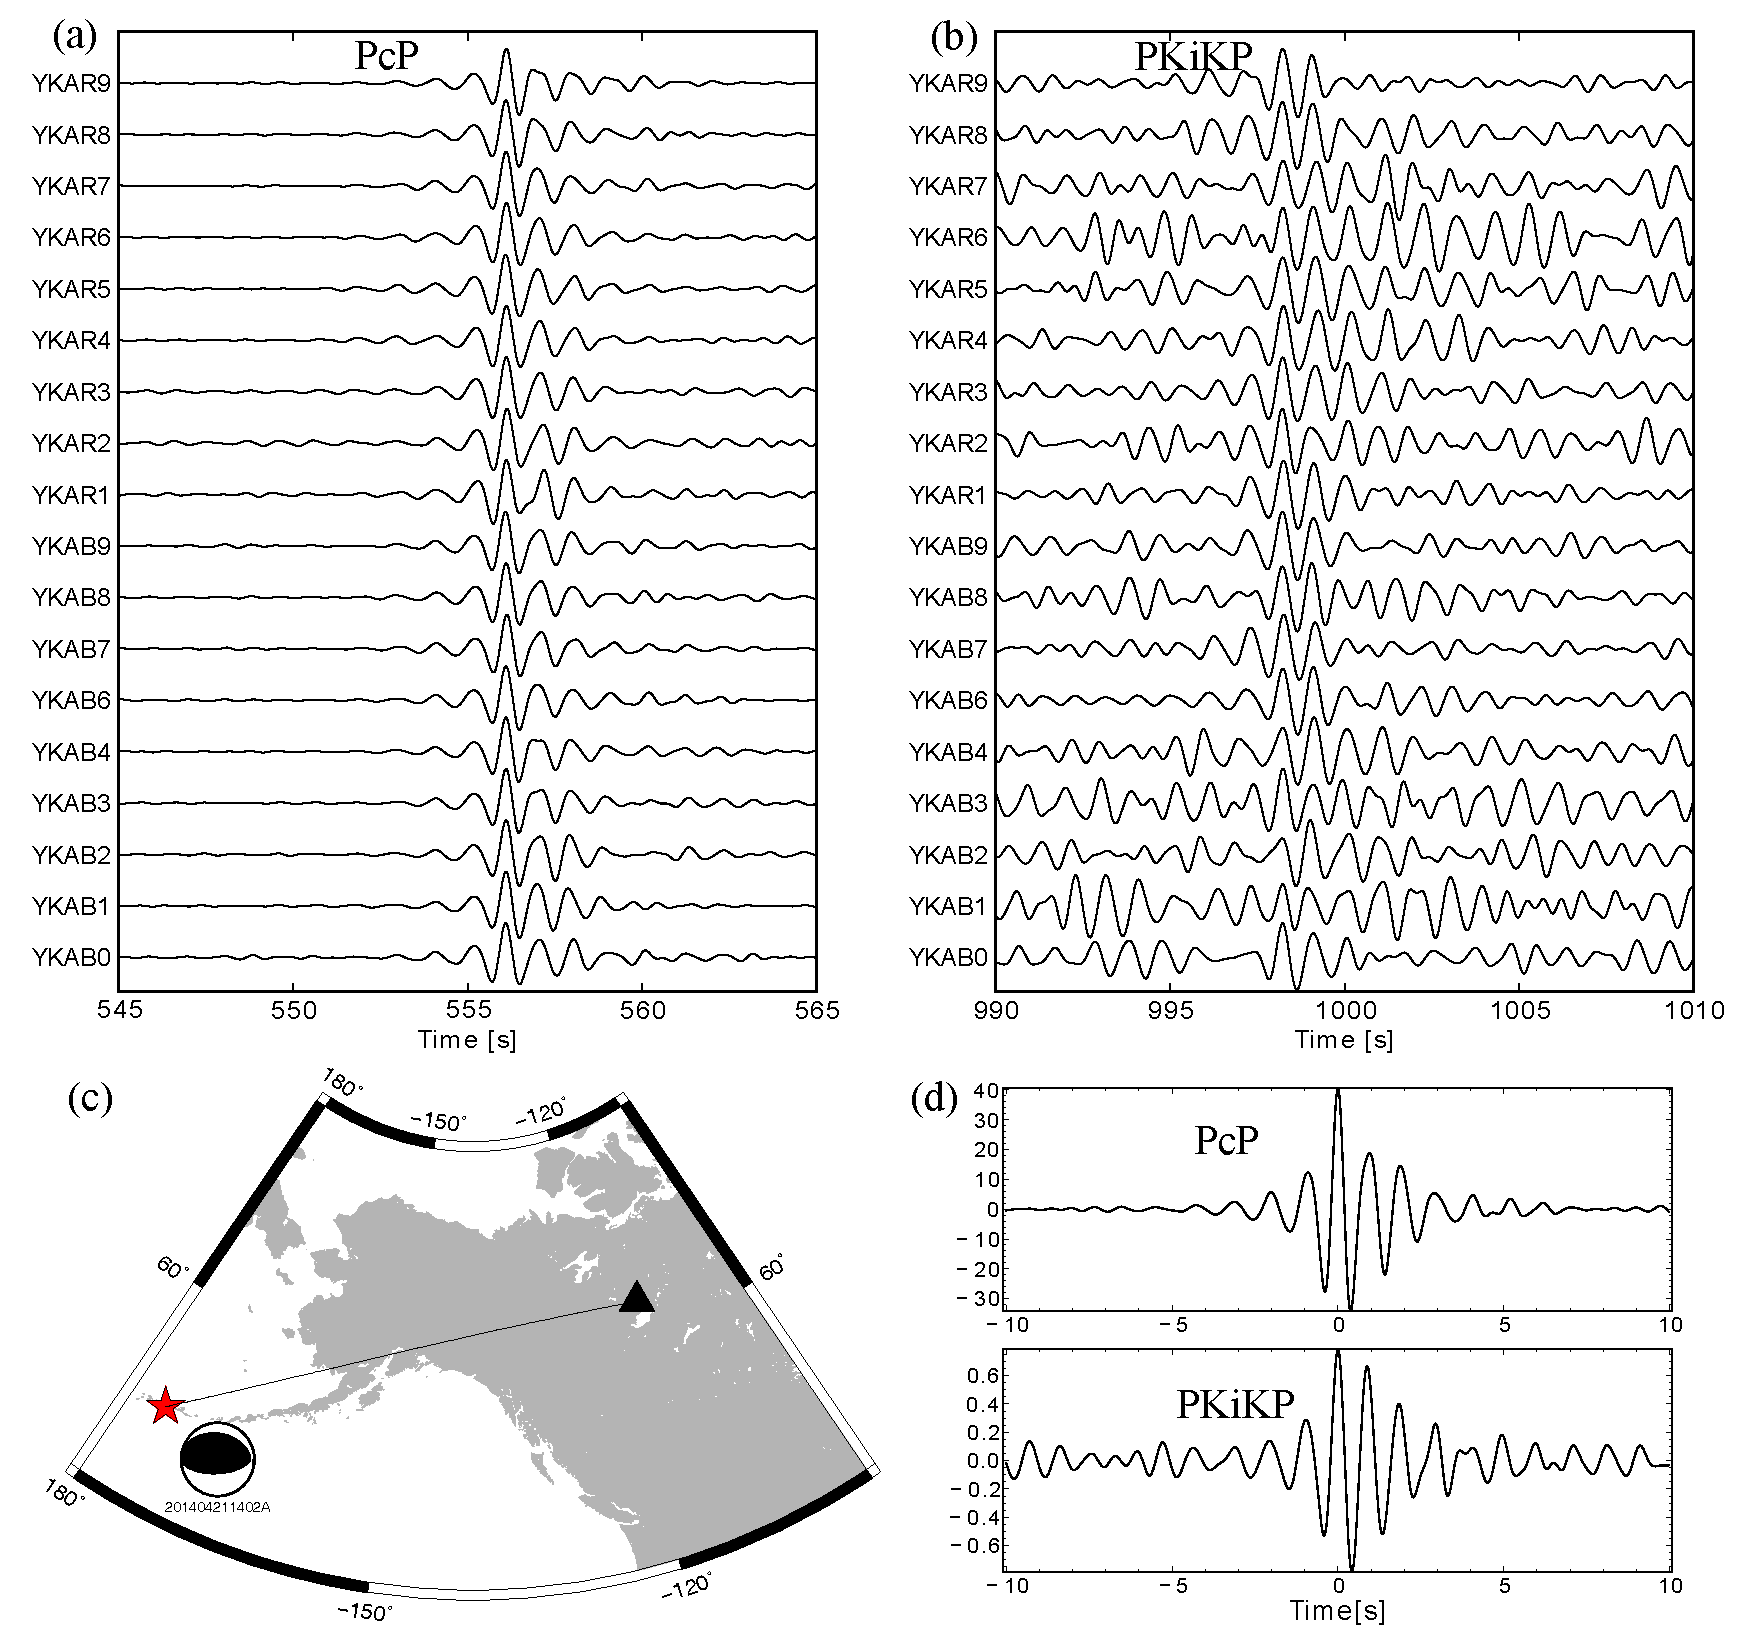
\includegraphics[width=\linewidth]{fig/chap2/4599655_yka}
\caption{YKA记录到的表\ref{evt}中事件10产生的PcP和PKiKP信号. (a) PcP;(b) PKiKP;(c)地震和台阵位置;(d) 按波峰对齐叠加后的PcP和PKiKP波形. }
\label{fig:4599655_yka}
\end{figure}

\begin{figure}
\centering
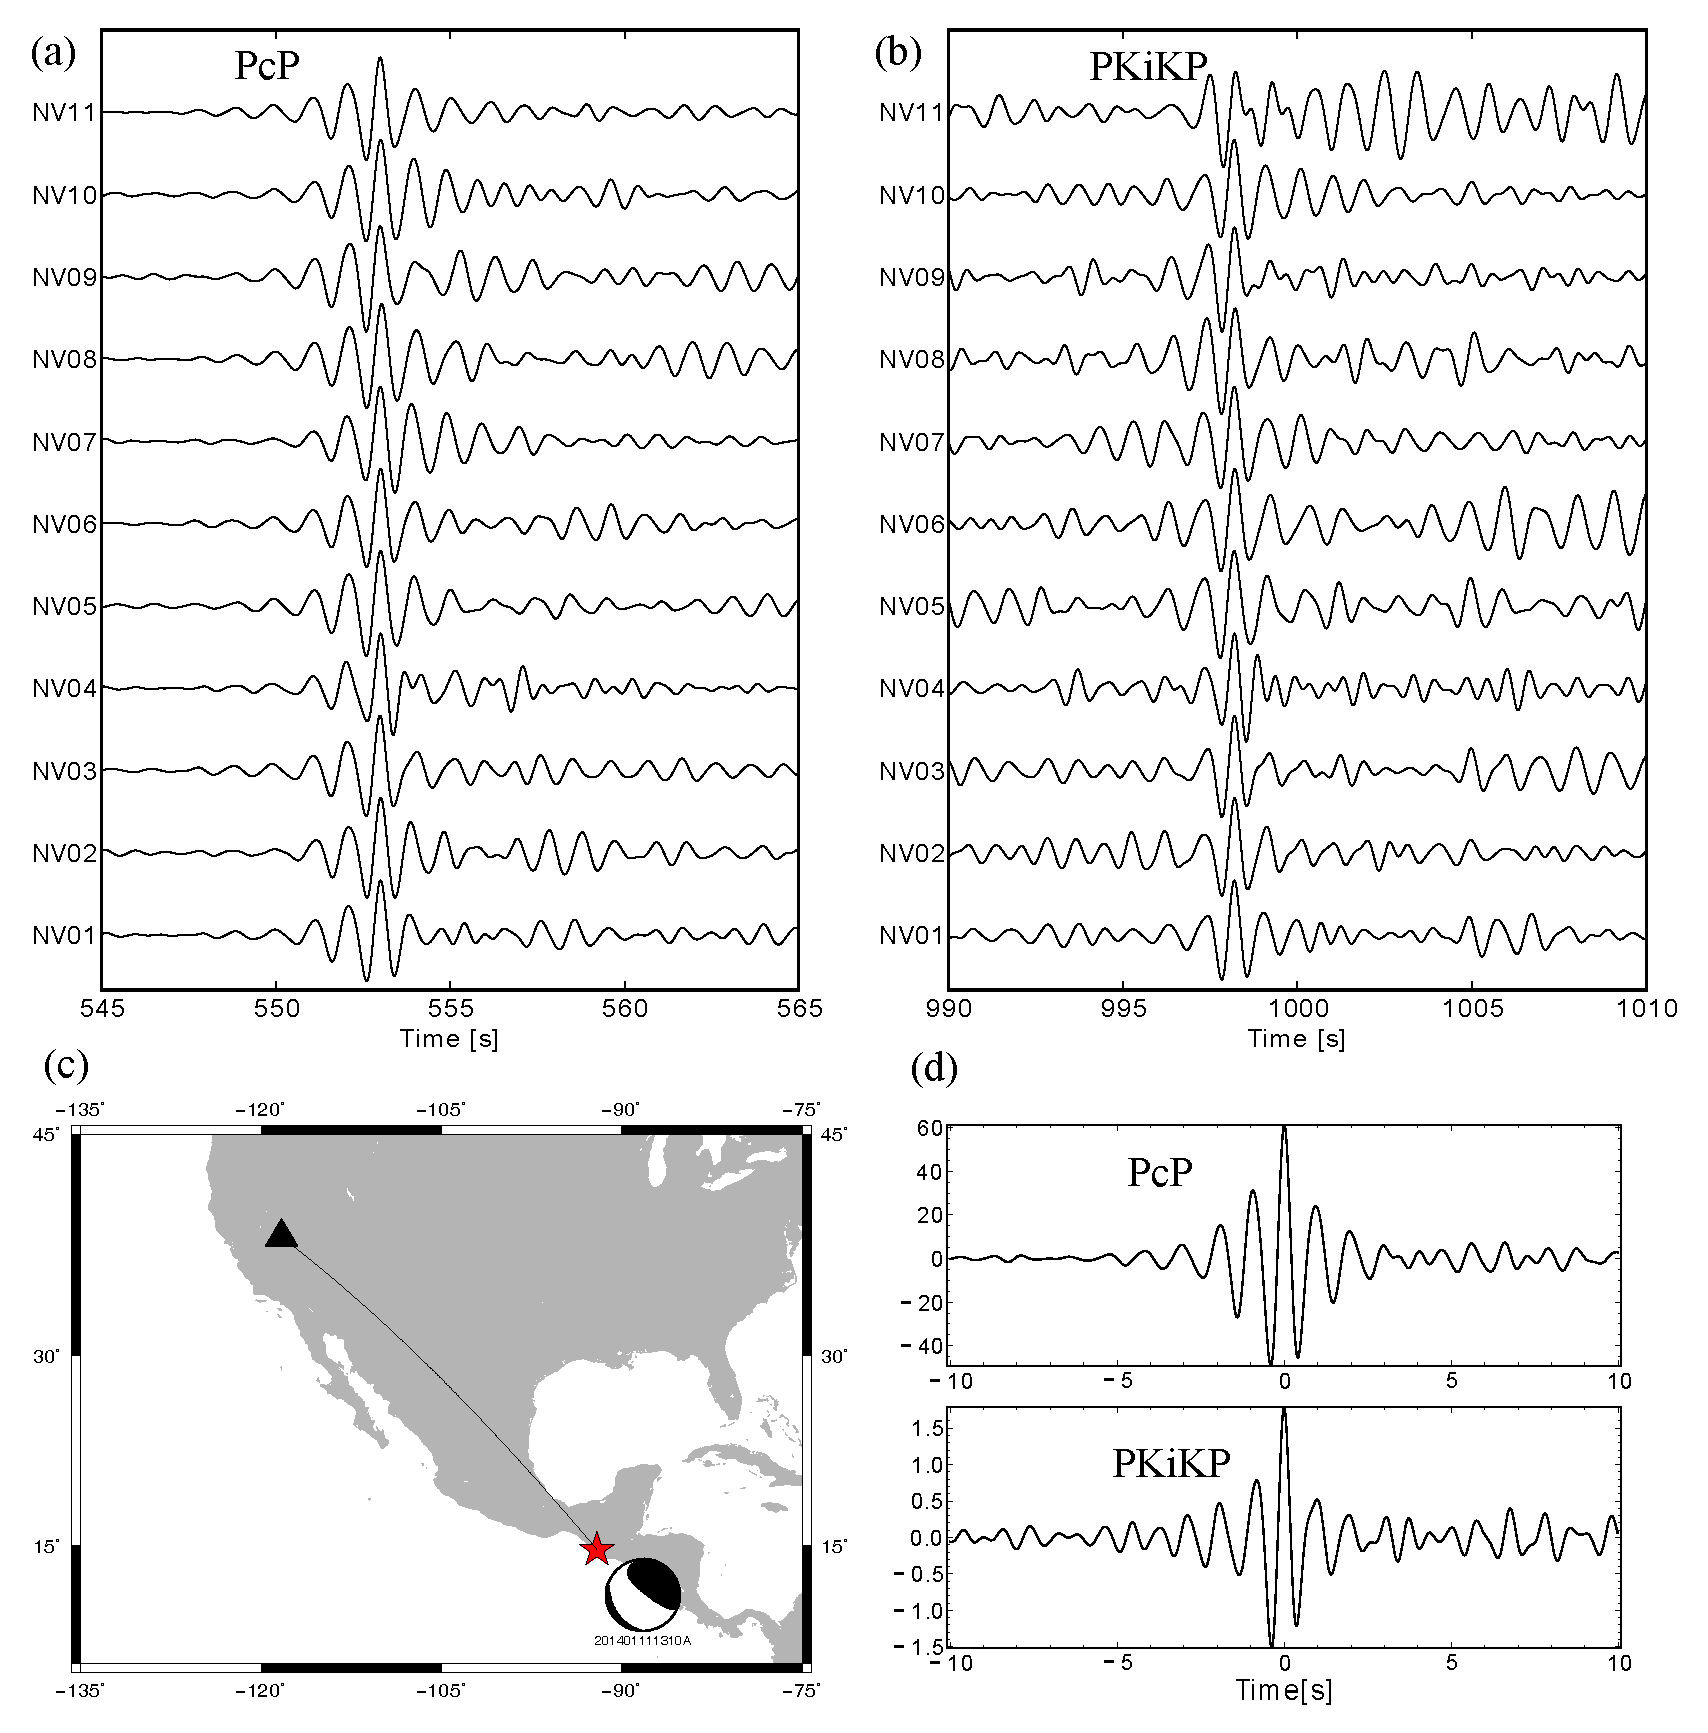
\includegraphics[width=1\linewidth]{fig/chap2/4371355_nvar}
\caption{NVAR记录到的表\ref{evt}中事件15产生的PcP和PKiKP信号. (a) PcP;(b) PKiKP;(c)地震和台阵位置;(d) 按波峰对齐叠加后的PcP和PKiKP波形. }
\label{fig:4371355_nvar}
\end{figure}

\begin{figure}
\centering
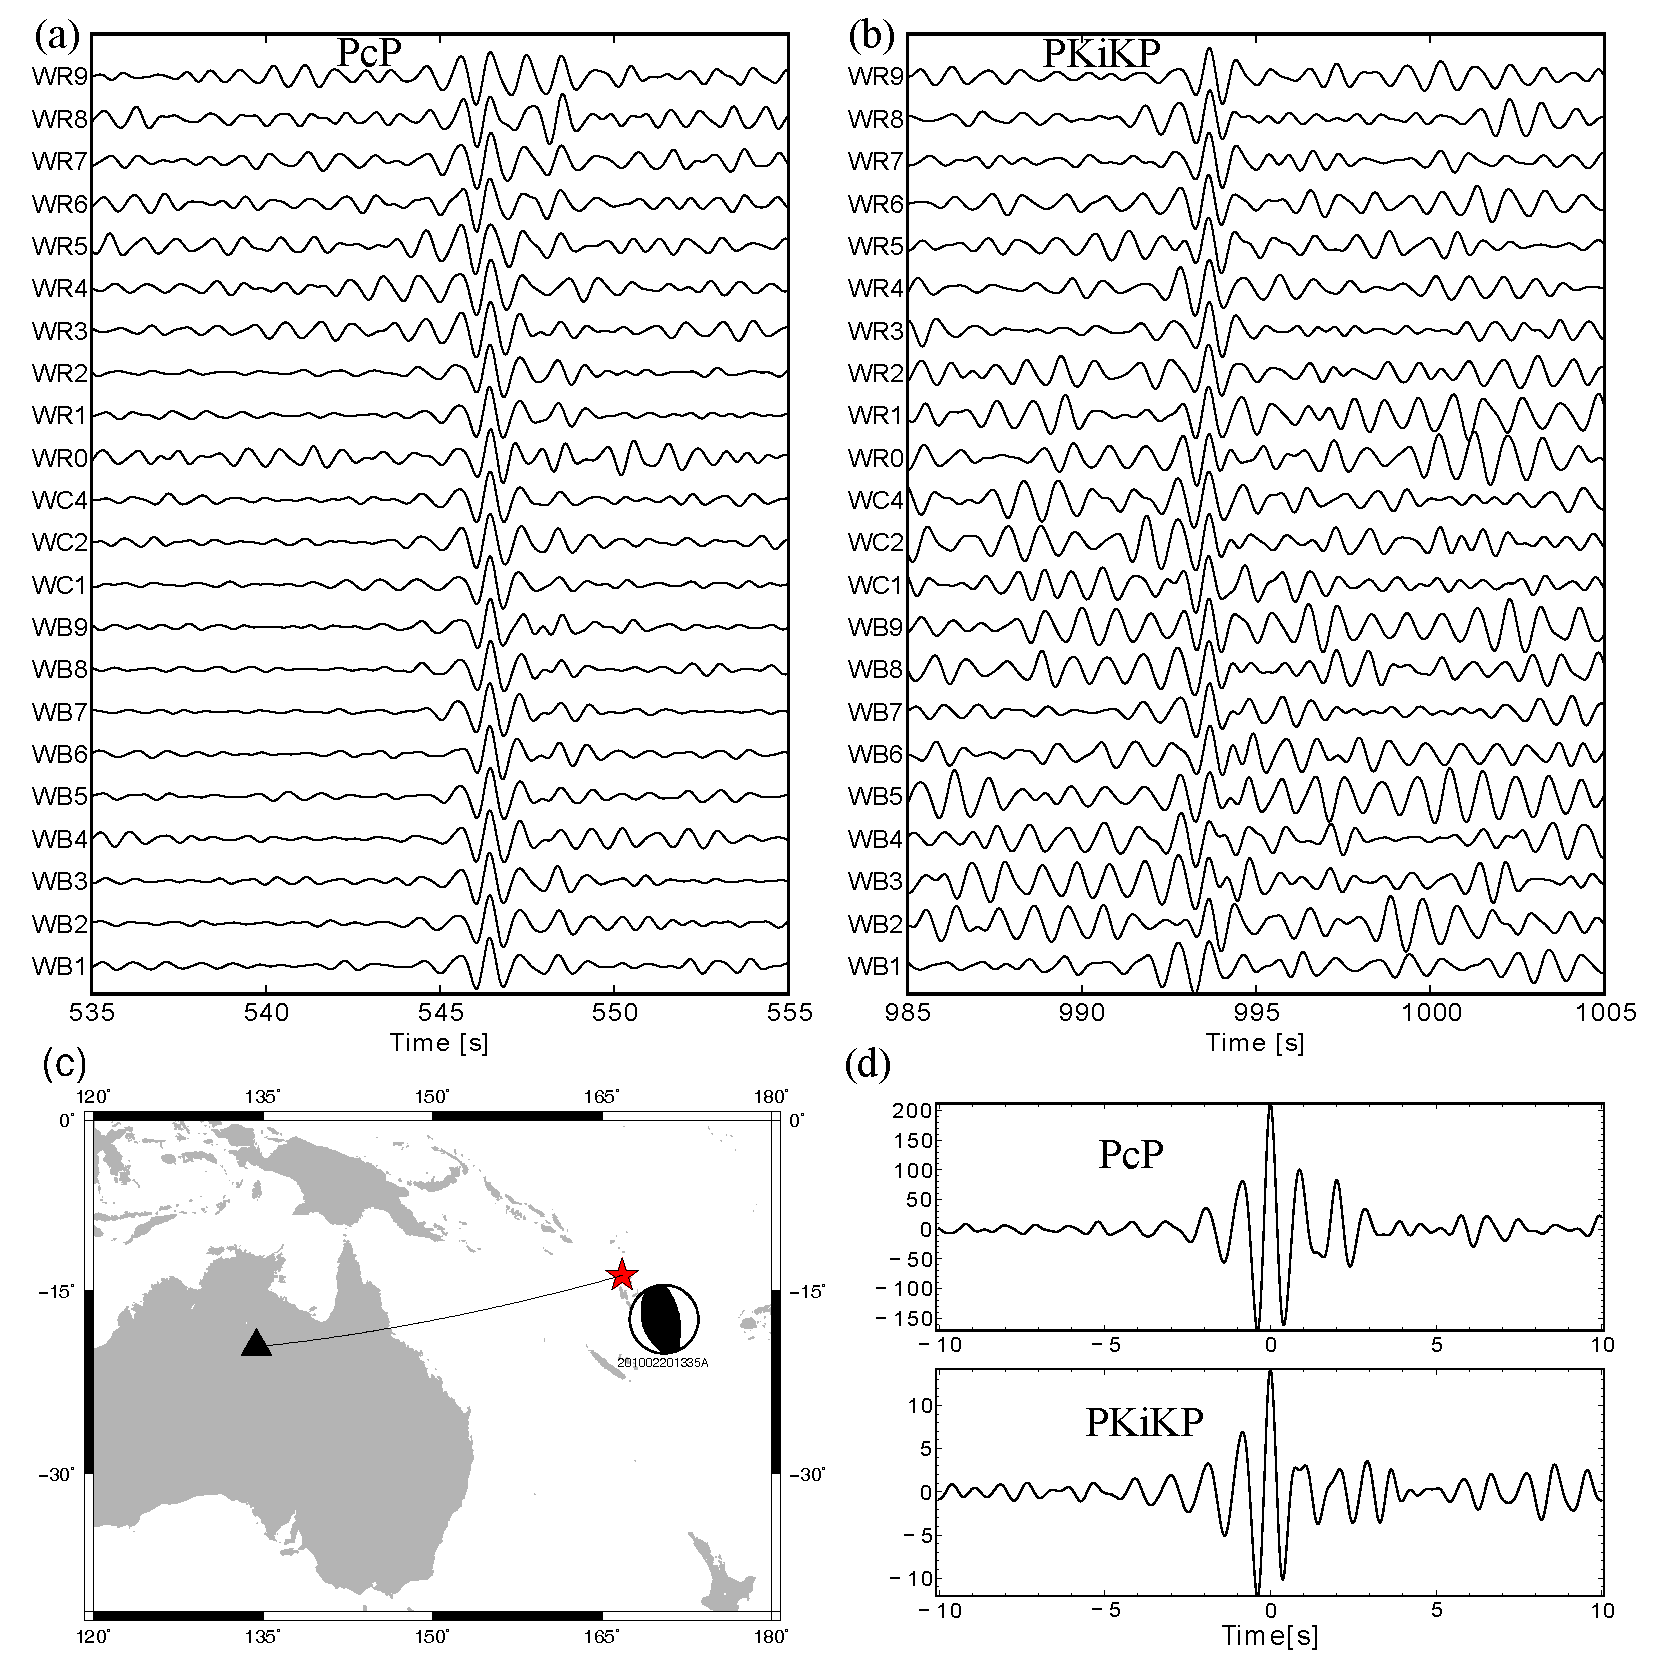
\includegraphics[width=1\linewidth]{fig/chap2/2844731_wra}
\caption{WRA记录到的表\ref{evt}中事件18产生的PcP和PKiKP信号. (a) PcP;(b) PKiKP;(c)地震和台阵位置;(d) 按波峰对齐叠加后的PcP和PKiKP波形. }
\label{fig:2844731_wra}
\end{figure}


由于IMS台阵的口径很小(一般为20km左右),每个台阵的台间距仅有几千米,因此可以减小单一台站产生的不确定性,比如由台站场地效应或者接收端下方的不均匀性造成的PcP和PKiKP振幅变化,并可以得到有效的观测质量评
价. 同时对PKiKP这样的弱震相的观测也将更加的可信,因为可以通过台阵叠加技术增加信噪比,对弱信号进行确认
,排除随机噪声的可能性~\citep{Rost2002},这一点将在后面进行详细叙述. 对所有的IMS数据,都经过去除仪器响应,并进行1--2Hz的四极Butterworth带通滤波. 根据前人的研究,这个频率范围是比较适合同时观测到PcP和PKiKP信号的~\citep{Koper2004a,Poupinet2004}. 在127个观测到PKiKP和PcP信号的地震之中,被两个台阵同时记录到这两个信号,且具有相近震中距情况的的只有30个左右,其中10个由NVAR和PDAR记录到(表\ref{evt},No.1--10);被WRA和ASAR记录的也有6个(表\ref{evt},No.17--23). 本文因此集中对这些地震的PKiKP和PcP数据进行分析. 

除了被两个台阵同时记录到的PcP和PKiKP数据,本研究还使用到了7个相邻地震产生的被同一个YKA台阵记录到的
PcP和PKiKP信号进行分析,来验证~\citet{Rost2004a}报道的阿拉斯加Kenai半岛下方CMB凹陷对PcP的放大效应. 这七个地震均位于阿留申群岛(表\ref{evt},No.11--17),与之前研究采样到相似的CMB区域. 

\begin{table}[ht]
	\centering
	\caption{本研究的对照分析所用到的所有地震.}
	\begin{tabular}{*{7}{c}}
	\hline
	事件号 & 日期 & 时间 & 纬度(\textdegree) & 经度(\textdegree) & 深度 & 震级(Mw)\\
	\hline
1 & 2003/08/25 & 06:28:34.9 &  13.9932 &  -91.1255 &  99.5 & 5.9\\
2 & 2007/07/23 & 22:30:09.2 &  14.465  &  -90.906  &  115  & 5.5\\
3 & 2009/11/26 & 19:08:10.4 &  13.4767 &  -89.9617 &  48.5 & 5.9\\
4 & 2009/04/27 & 16:46:27.5 &  16.9557 &  -99.5717 &  31.7 & 5.8\\
5 & 2009/05/03 & 16:21:46.4 &  14.6199 &  -91.2025 &  113.9 & 6.3\\
6 & 2009/08/15 & 13:22:43.1 &  18.0998 & -100.6157 &  61.2 & 5.5\\
7 & 2012/06/27 & 06:30:59.8 &  13.834  &  -89.967  &  132.6 & 5.7\\
8 & 2012/11/15 & 09:20:21.9 &  18.346  & -100.382  &  53  & 6.1\\
9 & 2013/07/08 & 02:52:42.6 &  13.2316 &  -89.1292 &  55  & 5.7\\
10 & 2014/01/11 & 13:10:51.1 &  14.6437 &  -92.0592 &  78  & 5.5\\
11 & 2015/04/23 & 14:57:27.7 &  51.7501 &  176.3353 &  31  & 5.3\\
12 & 2015/01/18 & 04:47:38.0 &  51.9238 &  179.578  &  102  & 5.5\\
13 & 2014/03/25 & 17:37:48.4 &  52.5754 & -177.1562 &  210.8 & 5.2\\
14 & 2007/07/13 & 21:54:44.9 &  51.904  & -176.2683 &  46.1 & 6.0\\
15 & 2014/04/21 & 14:02:15.8 &  51.844  & -175.9782 &  54.2 & 5.4\\
16 & 2009/04/21 & 08:37:28.8 &  52.2147 & -173.3826 &  68.3 & 5.2\\
17 & 2009/01/26 & 19:11:48.2 &  52.0884 & -171.3288 &  32.9 & 5.7\\
18 & 2010/02/20 & 13:35:57.1 & -13.6853 &  166.7666 &  87.3 & 5.5\\
19 & 2010/06/17 & 13:06:51.3 & -33.1905 &  179.7819 &  211.2 & 6.0\\
20 & 2011/01/26 & 17:03:30.1 & -11.0379 &  166.3601 &  153.5 & 5.8\\
21 & 2007/08/19 & 13:44:06.0 & -20.6189 &  169.7323 &  89.7 & 5.6\\
22 & 2007/11/20 & 15:28:28.6 & -29.973  & -177.9397 &  57.8 & 5.9\\
23 & 2007/10/11 & 05:31:55.6 & -18.5046 &  168.991  &  214  & 5.4\\
	\hline
\multicolumn{7}{l}{\footnotesize{注:1--10,11-17和18-23号事件分别用于后面三个区域的分析.}}
\end{tabular}
\label{evt}
\end{table}

\subsection{大型台网}

本研究还利用全球现有的大型台网增大PKiKP和PcP的观测数量,以此补充IMS小口径台阵的数据并增大采样区域,试图探索大尺度下的CMB或者ICB变化. 对于北美的NVAR和PDAR,它们记录到表\ref{evt}中地震2和3的时刻,美国的流动台网USArray恰好分别移动到这两个台阵附近,这样就提供了一个很好的机会比较两个数据集,进一步验证IMS台阵的观测结果. 虽然USArray台站的信噪比不如IMS台阵,但仍然有一些清晰的PKiKP和PcP观测. 

\begin{figure}[ht]
		\centering
		\subfloat[PKiKP]{\label{pkikp11}%
		\includegraphics[width=0.45\linewidth,height=0.4\textheight]{fig/chap2/pkikp_sec_2011.eps}
		}
		%\hspace{1em}
		\subfloat[PcP]{\label{pcp11}%
		\includegraphics[width=0.45\linewidth,height=0.4\textheight]{fig/chap2/pcp_sec_2011.eps}
		}
		\caption{国家测震台网记录到的事件2011/02/04 13:53:46(Dep=86km,Mw6.3)产生的549道单道可见的PKiKP\subref{pkikp11}信号,对应的PcP\subref{pcp11}也比较明显,但在某些区段看不到PcP信号. }
		\label{cn_2011}
\end{figure}


\begin{figure}
\centering
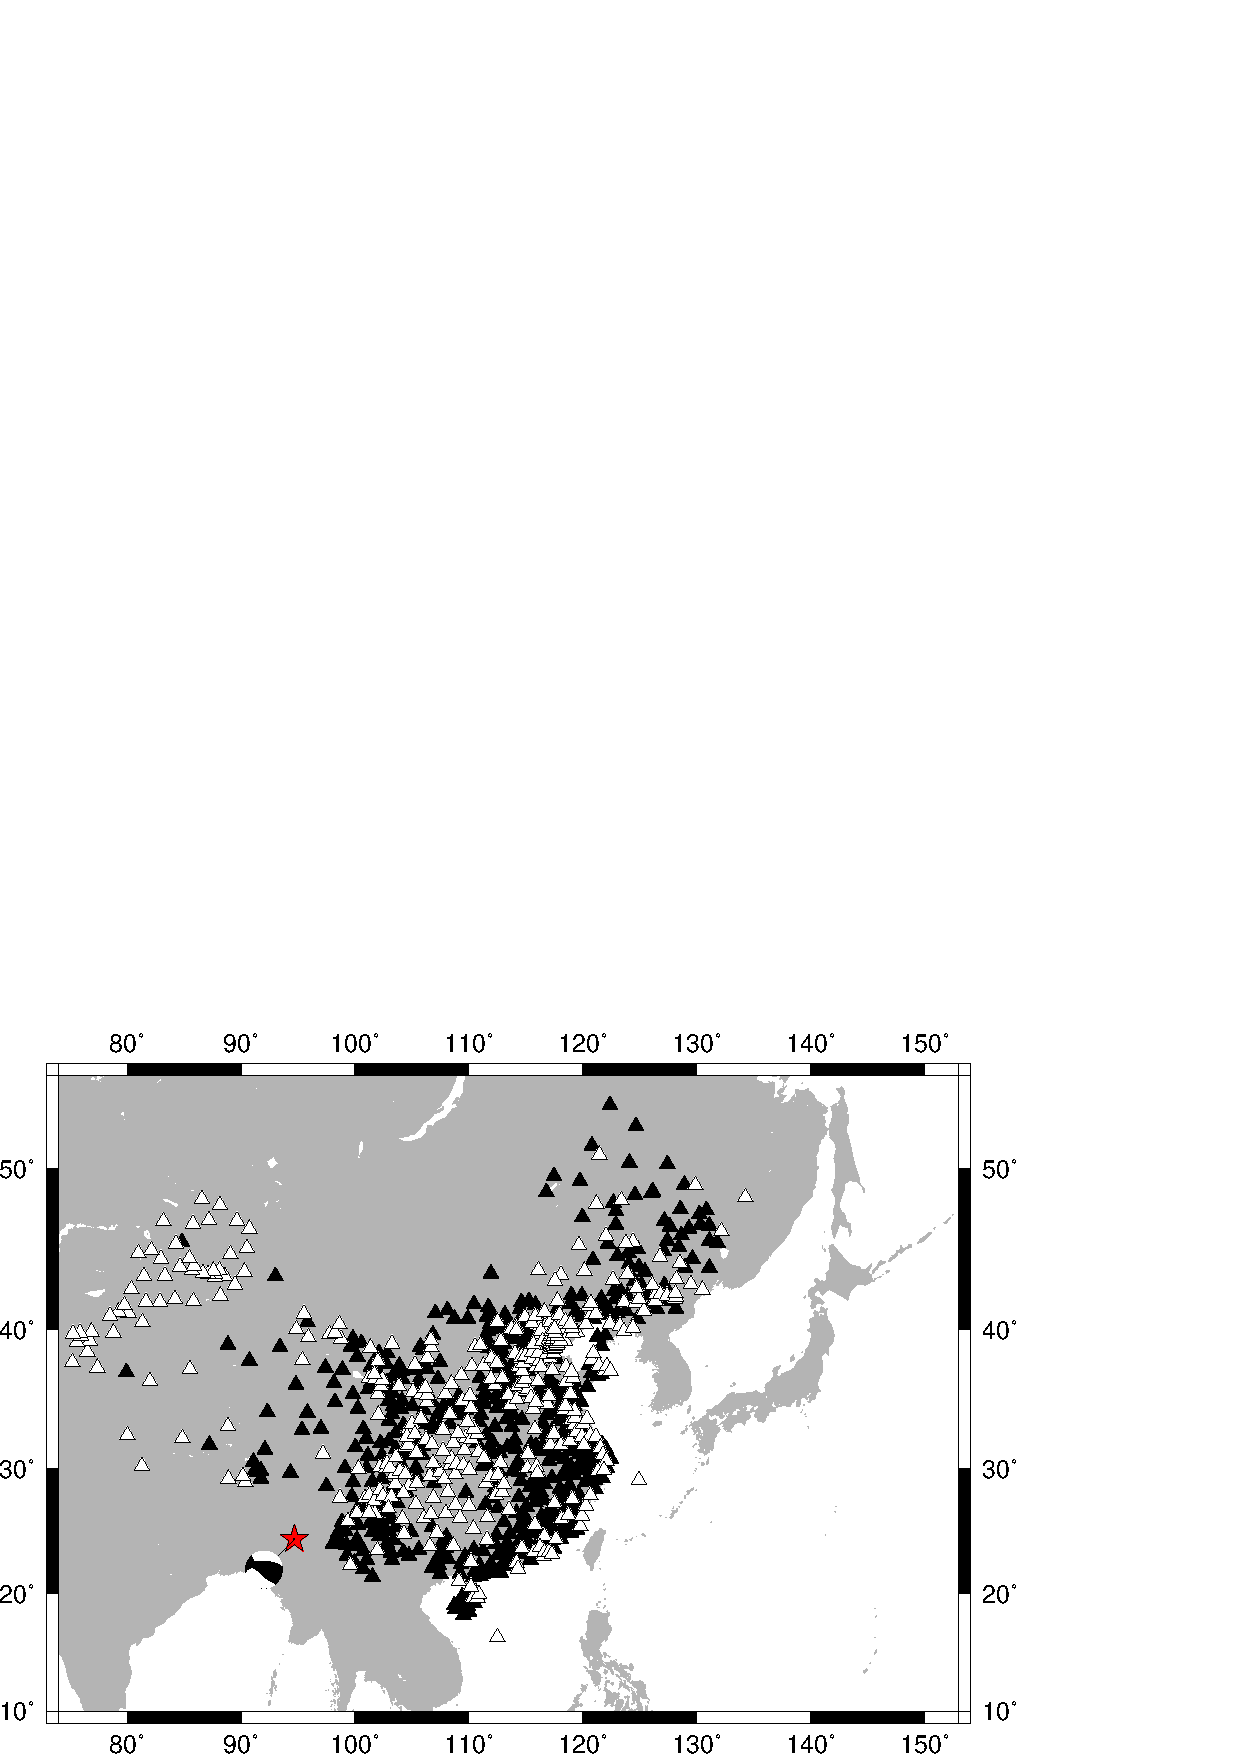
\includegraphics[width=0.8\linewidth]{fig/chap2/ev_sta_2011}
\caption{图\ref{cn_2011}中记录对应的台阵分布和地震位置. 黑色三角形表示记录到PKiKP信号的台站,白色的表示未记录到PKiKP信号的台站.}
\label{fig:ev_sta_2011}
\end{figure}


\begin{figure}[ht]
		\centering
		\subfloat[PKiKP]{\label{pkikp13}%
		\includegraphics[width=0.45\linewidth,height=0.4\textheight]{fig/chap2/pkikp_sec_2013.eps}
		}
		%\hspace{1em}
		\subfloat[PcP]{\label{pcp13}%
		\includegraphics[width=0.45\linewidth,height=0.4\textheight]{fig/chap2/pcp_sec_2013.eps}
		}
		\caption{国家测震台网记录到的事件2013/05/24 14:56:30(Dep=630km,Mw6.7)产生的513道单道可见的PKiKP\subref{pkikp13}信号,对应的PcP\subref{pcp13}也比较明显,但在某些区段看不到PcP信号. }
		\label{cn_2013}
\end{figure}


\begin{figure}
\centering
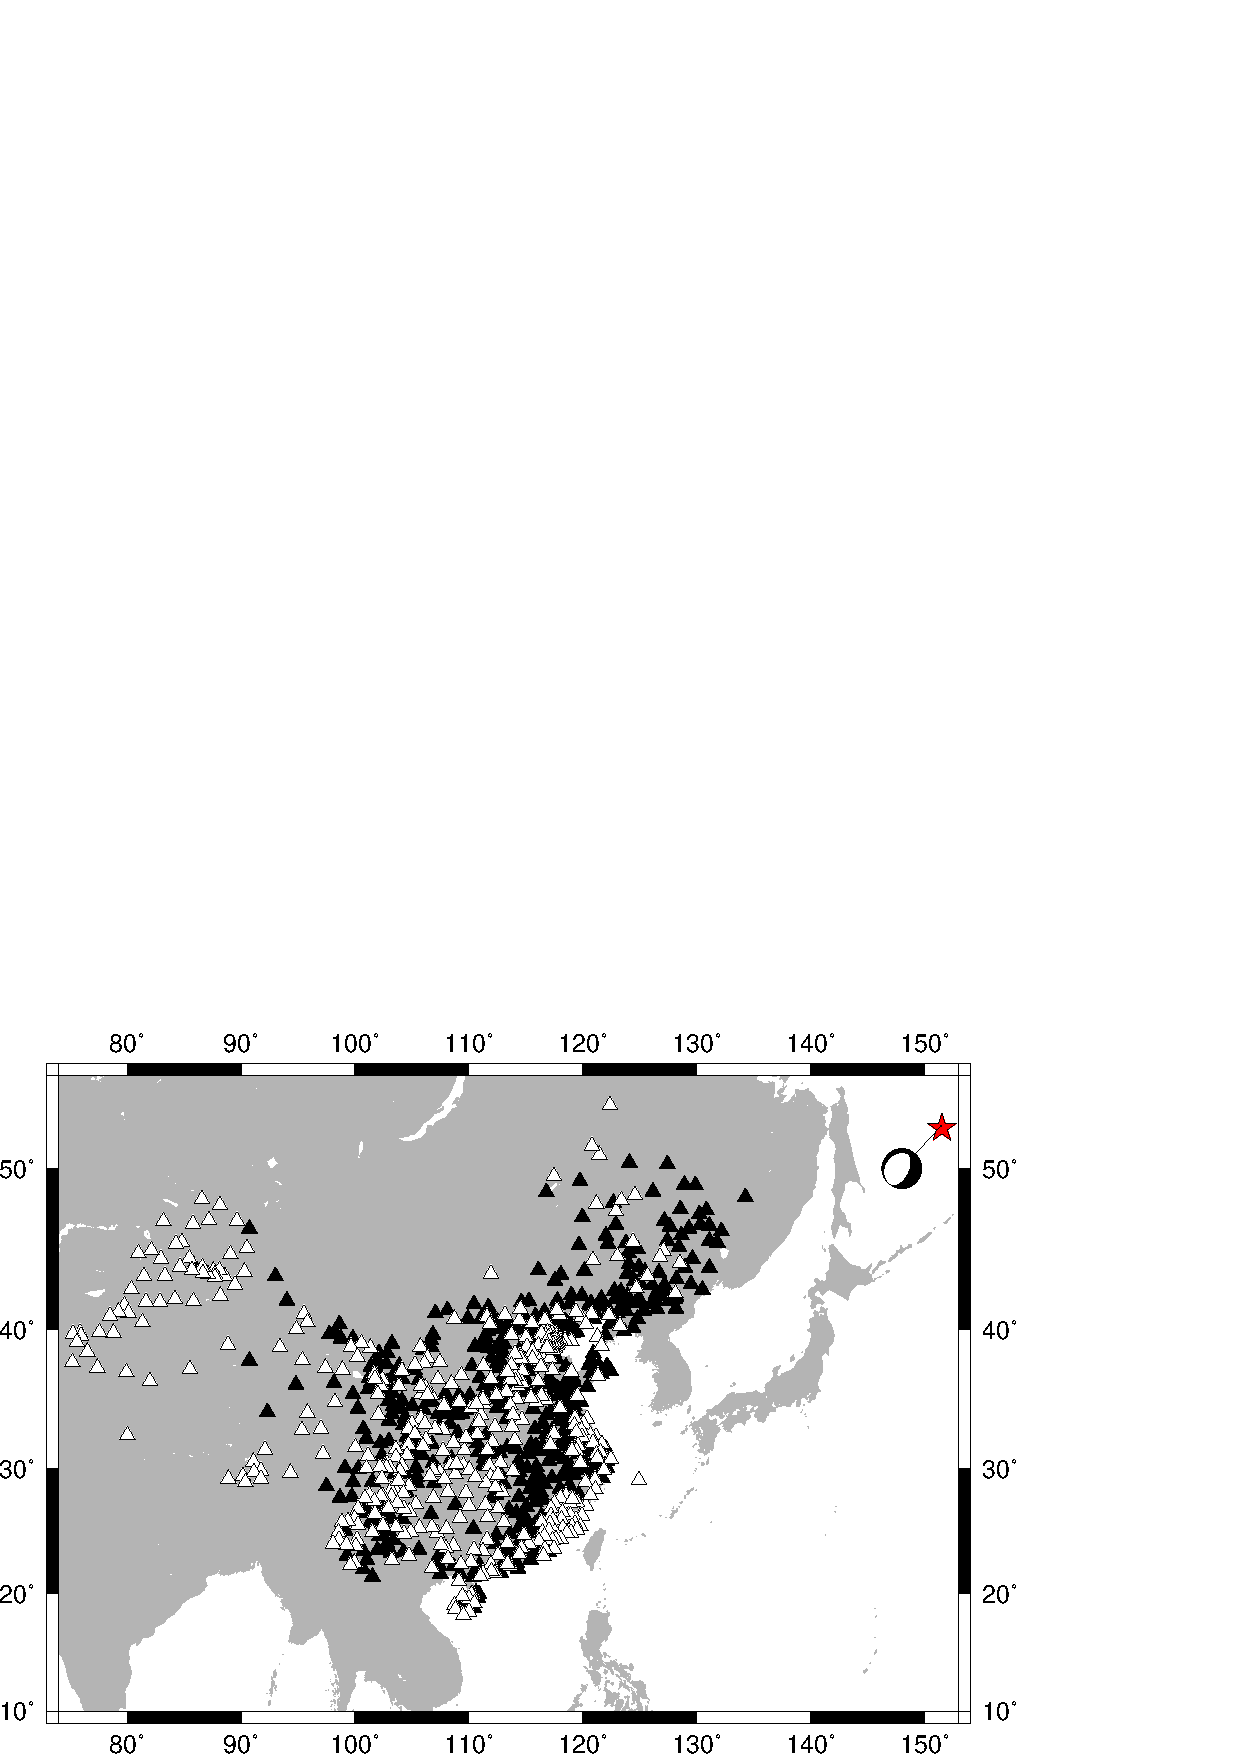
\includegraphics[width=0.8\linewidth]{fig/chap2/ev_sta_2013}
\caption{图\ref{cn_2013}中记录对应的台阵分布和地震位置. 黑色三角形表示记录到PKiKP信号的台站,白色的表示未记录到PKiKP信号的台站.}
\label{fig:ev_sta_2013}
\end{figure}

由于缺少东亚的IMS台站数据,这里用日本Hi-net台网和国家测震台网对东亚下方的CMB/ICB进行补充采样. 由于这些密集台网的台站数量均超过700个,所以不便用来搜索PKiKP观测. 于是本研究采用先用单个稳定的固定台先对附近的地震事件进行搜索,找到能产生PKiKP的事件,这里使用牡丹江台(MDJ)进行搜索近二十年的地震事件. 使用这种方法,利用国家测震台网观测到两个产生500个以上清晰PKiKP信号的地震事件,这在世界上也是首次得到如此连续的跨度达到40{\textdegree}震中距的记录(图\ref{cn_2011}和图\ref{cn_2013}). 尤其值得注意的是图\ref{cn_2011}中云南台网记录到的小于4{\textdegree}的清晰PKiKP波形,如此小震中距下仍然有清晰的内核反射震相,暗示了尖锐ICB的存在. 要产生大量的PKiKP反射必然要满足很多条件,首先必须要有足够大的震级激发出足够强的PKiKP信号,这两个地震均超过6级,相比而言,由牡丹江台搜索出的其他较小震级地震就没能产生类似的PKiKP观测数量;其次,地震需要有合适的震源辐射花样,PKiKP的离源角应该指向辐射能量大的方向,通过Harvd全球CMT解(\url{http://www.globalcmt.org/})计算,这也得到了验证(图\ref{fig:rad});除了震源因素,台阵场地效应、台阵周围的噪声环境都能影响PKiKP的观测. 就以上两个地震而言,中国中部普遍缺少PKiKP观测(图\ref{fig:ev_sta_2011},\ref{fig:ev_sta_2013}),正是源于台站下方的沉积层对PKiKP能量的衰减作用,而位于山地的台站,由于其台基在基岩之上,普遍都有清晰的PKiKP记录.


 

\begin{figure}[ht]
\centering
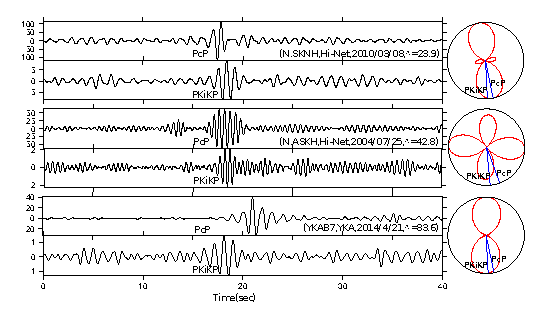
\includegraphics[width=0.8\linewidth]{fig/chap2/rad}
\caption{Hi-net和YKA台站记录到的三个不同震中距地震事件产生的PcP、PKiKP波形(左),和对应的P波辐射花样(右). 在小震中距情况下两者的离源角相差不大(上、下),当震中距增大时PcP和PKiKP的辐射能量有明显差异(中). }
\label{fig:rad}
\end{figure}


\section{数据处理方法}

这一节介绍研究中的数据处理方法. 包括搜索PKiKP信号用到的叠加方法,计算台阵平均PKiKP/PcP振幅比和平均差异走时残差的方法以及数据筛选的一些准则. 

\subsection{PKiKP信号的预识别}

如前文所提到,本研究需要从全球的IMS台阵数据中挑选可识别的PKiKP信号,但是人工挑选由于可能存在的肉眼识别偏差,会遗漏某些产生PKiKP信号的地震事件,虽然单个台站记录不太明显,但叠加后的波形却十分清晰. 本文所使用的均是能产生清晰叠加结果的记录,叠加方法使用的是PWS. 

PWS方法最早见于地幔间断面转换波的探测~\citep{Schimmel1997},能够增强连续的一致信号,压制不连续的随机噪声,目前较为广泛地用于弱信号的识别. 典型的例子就有其应用于前临界PKiKP的研究
~\citep{Koper2003,Koper2004},还有用于寻找穿过内核的S波震相PKJKP~\citep{Deuss2000}以及识别在内核内侧反射的PKIIKP震相~\citep{Niu2008}. 下面将简要介绍PWS方法的原理和其叠加效果. 

PWS是一种非线性叠加方法,它使用一种不依赖振幅的一致性度量方法来加权线性叠加. 在叠加的过程中
首先要构建一个解析复信号$S(t)$,它的实部是台站接收到的信号$s(t)$,虚部是则是实部的希尔伯特
变换

\begin{equation}
S(t) = s(t) + i \mathscr{H} [s(t)]
\end{equation}

上式可以写成振幅和震相分离的形式

\begin{equation}
S(t) = A(t) exp[i \Phi (t)]
\end{equation}

其中$A(t)$是地震信号的波包,$\Phi (t)$为瞬时震相. 震相叠加的表达式如下

\begin{equation}
c(t) = \frac{1}{N} \left| \sum_{j=1}^{N} exp[i \Phi_j (t)] \right|
\end{equation}

用震相的$\nu$次幂作为加权系数,就得到了PWS的表达式

\begin{equation}
 \nu_{PWS}(t) = \frac{1}{N} \sum_{j=1}^{N} s_j (t)c^{\nu} (t)
\end{equation}

当加权系数取0的时候即为常规的线性叠加,本研究中PWS加权系数均取2. 除此之外,在预挑选过程中不做慢度偏移,直接进行零慢度叠加. 首先,这样给数据处理带来了方便;其次,IMS台阵的口径都很小,对慢度的分辨能力很低~\citep{Rost2002},零慢度叠加常常就能得到很好的效果. 图\ref{fig:stack}分别对比了YKA台阵中对某个地震事件的单台记录、线性叠加和PWS叠加结果. 可以明显看出,叠加之后的微弱PKiKP信号明显增强. 这里需要特别提到,这里的叠加仅仅是为了对地震事件进行挑选,由于叠加之后的的振幅并不能体现出真实的振幅信息,因此不参与后面的振幅比计算. 

\begin{figure}
\centering
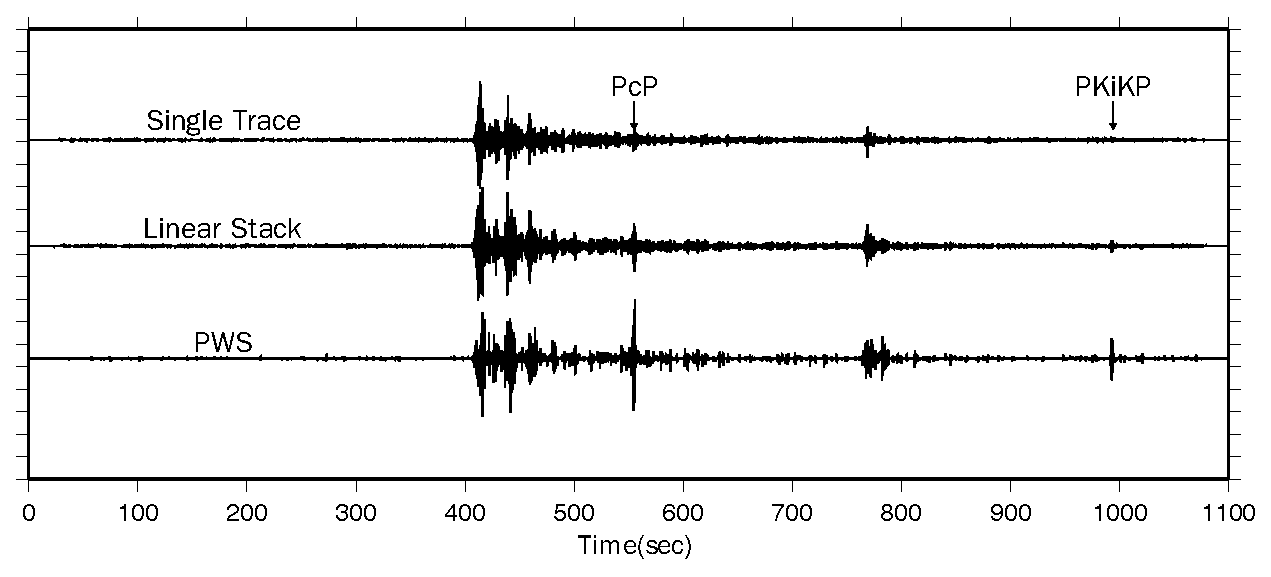
\includegraphics[width=0.8\linewidth]{fig/chap2/stack}
\caption{YKA台阵对事件2014/06/03,22:29:51(106 km, Mb6.0)的单道记录和叠加结果比较. 图中上为台阵中某单道记录,中间为线性叠加结果,下为PWS处理后的结果. }
\label{fig:stack}
\end{figure}

\subsection{振幅比和走时残差的计算}

\subsubsection{PKiKP/PcP振幅比}

前人利用IMS台阵数据研究内核边界通常使用的是所有台站记录经过线性叠加后得到叠加记录的PKiKP/PcP振幅比,最终每一个事件-台阵对就仅只剩下一个振幅比数据~\citep{Koper2004a}. 这样做虽然得到了一个平均的比值,但却丢失了很多信息. 因为即使是口径仅20千米的小口径台阵,每个台阵的记录差别可能依然会很大,而且尤其
体现在PcP的振幅差别上,因为PcP比PKiKP更容易受到浅层结构的影响. 产生差别的原因有很多,其中一个比较重要的
就是每个台站下方的物性差异. 比如,台站下方介质比较致密的岩石的台站记录到的PcP振幅就会比下方是松软沉积
层的台站记录到要大. 如果仅仅做简单的叠加,得到的振幅比可能与真实值相差很大,同时也不能得到振幅比测量
值的可信度估计. 

考虑到台阵内存在的不确定性,本研究采用计算台阵平均振幅比的方法,即先计算台阵内每个台站的PKiKP/PcP振幅比然后再计算所有台站的平均值. 假设台阵内的台站数为$N$,第$i$个台记录的PcP和PKiKP振幅分别为$A_i^{PcP}$和$A_i^{PKiKP}$,则该台的振幅比为

\begin{equation}
r_i = \frac{A_i^{PKiKP}}{A_i^{PcP}}
\end{equation}

于是可以得到台阵的平均振幅比

\begin{equation}
\overline{r} = \frac{1}{N} \sum_{i=1}^{N} r_i
\end{equation}

还可计算每个台阵振幅比的标准差,用于振幅比测量的可靠性评价

\begin{equation}
\sigma = \sqrt{\frac{\sum_{i=1}^{N} (r_i - \overline{r} )}{N}}
\end{equation}

虽然采用台阵平均振幅比有其优越性,但有的时候测量每个台阵的振幅比却会遇到困难,因为当信噪比过低的时候相
位的振幅不容易读出来. 因此关于每道记录的PKiKP/PcP振幅测量,采用如下方法:首先根据预叠加结果找到震相
最大振幅的位置,然后在所有台站记录中找到质量最好震相的最大振幅峰值位置,再对其他各道记录注意追踪震相,
以其峰值作为振幅,如果不能追踪,则剔除该道记录. 当然,对于每道记录,这个峰值并不一定是该信号的最大振幅
值,但即使这样也并不会有太大差异,而且这些差异都最终体现在平均振幅比的标准差上. 

前面提到在震中距较大时PcP和PKiKP离源角有比较大的差异,因此需要做震源辐射校正,否则可能对后续的振幅比分析产生影响. 根据~\citep{Aki2002a},远场P波辐射花样可以表示为,

\begin{equation}
\mathcal{F}^P = \bm{\gamma} \cdot \bm{M} \cdot \bm{\gamma}
\end{equation}

其中$\bm{M}$是矩张量,而$\bm{\gamma}$为P波极化方向,可以用离源角$i_{\xi}$和方位角$\phi$表示

\begin{equation}
\bm{\gamma} = \left(\begin{array}{c}
\sin i_{\xi} \cos \phi \\
\sin i_{\xi} \sin \phi \\
\cos i_{\xi}
\end{array}\right)
\end{equation}

做震源辐射校正即将关测的振幅比乘上PcP和PKiKP辐射因子的比值%
$\frac{\mathcal{F}^{PcP}}{\mathcal{F}^{PKiKP}}$. 

\subsubsection{PKiKP-PcP走时残差}

对于PKiKP-PcP走时残差,其计算方法和台阵平均振幅比类似,也是先得到每一个台站的走时残差,再计算整个台
阵的平均值. 本研究中,PcP和PKiKP的走时差均认为是其峰峰或者谷谷的时差;残差则是相对于PREM而言,这是
因为在该模型的构建过程中加入了PcP-PKiKP走时观测结果,使得其与实际观测资料能有比较好的拟合度. 影响PK
iKP-PcP走时残差的影响因素除了相对PREM的局部的内外核厚度变化,还有地球的椭率和两个震相经过的地幔部分
速度的差异. 但在本研究中不考虑后两种因素,首先本研究分析所用的IMS台阵数据采样的CMB区域非常小,因此假
定这两个因素对残差的贡献很小. 而且分析考虑的是走时残差的相对变化,并由此推测CMB的小尺度结构,所以走时
残差仅做如下计算,

\begin{equation} T_{res} = (T_{PKiKP}^{obs} - T_{PcP}^{obs}) - (T_{PKiKP}^{prem} - T_{PcP}^{prem})
\end{equation}

相比与台阵平均振幅比的不确定性, 每个台站的相对走时残差的差异都很小,平均走时残差的标准差一般为0.01秒的量级,这也体现出走时观测比振幅观测要稳定可靠得多. 